\documentclass[a4paper,10pt,oneside]{scrreprt}
\usepackage[latin1]{inputenc}
\usepackage[english]{babel}
\usepackage{graphicx}
\usepackage{float}
\usepackage{geometry}
\geometry{verbose,a4paper,tmargin=15mm,bmargin=25mm,lmargin=15mm,rmargin=15mm}
\usepackage{paralist}

\usepackage{paracol}

\usepackage{todonotes}

\usepackage{listings}
\lstset{language=Java,
	tabsize=2,
	showspaces=false,
	showtabs=false,
	breaklines=true,
	showstringspaces=false,
	breakatwhitespace=true,
	commentstyle=\color{pgreen},
	keywordstyle=\color{pblue},
	stringstyle=\color{pred},
	basicstyle=\footnotesize\ttfamily,
	moredelim=[il][\textcolor{pgrey}]{$$},
	moredelim=[is][\textcolor{pgrey}]{\%\%}{\%\%}
}

\usepackage{tikz}
\usetikzlibrary{calc,patterns,angles,quotes}

\usepackage{caption}
\usepackage{subcaption}
\usepackage{tabularx} % in the preamble

\usepackage{pdfpages}

%\usepackage{indentfirst} % for always indenting the first paragraphs

\usepackage{wrapfig}
\usepackage{lipsum}
\usepackage[linewidth=1.2pt,linecolor=red]{mdframed} % for boxes around wrapfigure and text

\begin{document}


\begin{center}
	Submitted by Group 18

	\bigskip

	\begin{tabular}{c}
	Group Members: \\
	CETIN, Ulfet (391819); GRUCZKA, FILIP (413279);	LIPINSKI, Bartosz (413177) \\
	SZYMANSKI, Bartosz (411949); GONG, Zeheng (378125)\\
	\end{tabular}

	\bigskip

	DIS1 WS 19/20 - Project Milestone III\\
	Ideation - Phase II\\

	%	(ordered on lastname basis)
\end{center}
\vspace{-1cm}

\clearpage

\begingroup
\let\clearpage\relax
	\chapter{Storyboard walkthrough}
\endgroup


\section{Solution \#1:}

\begin{figure}[H]
	\centering
	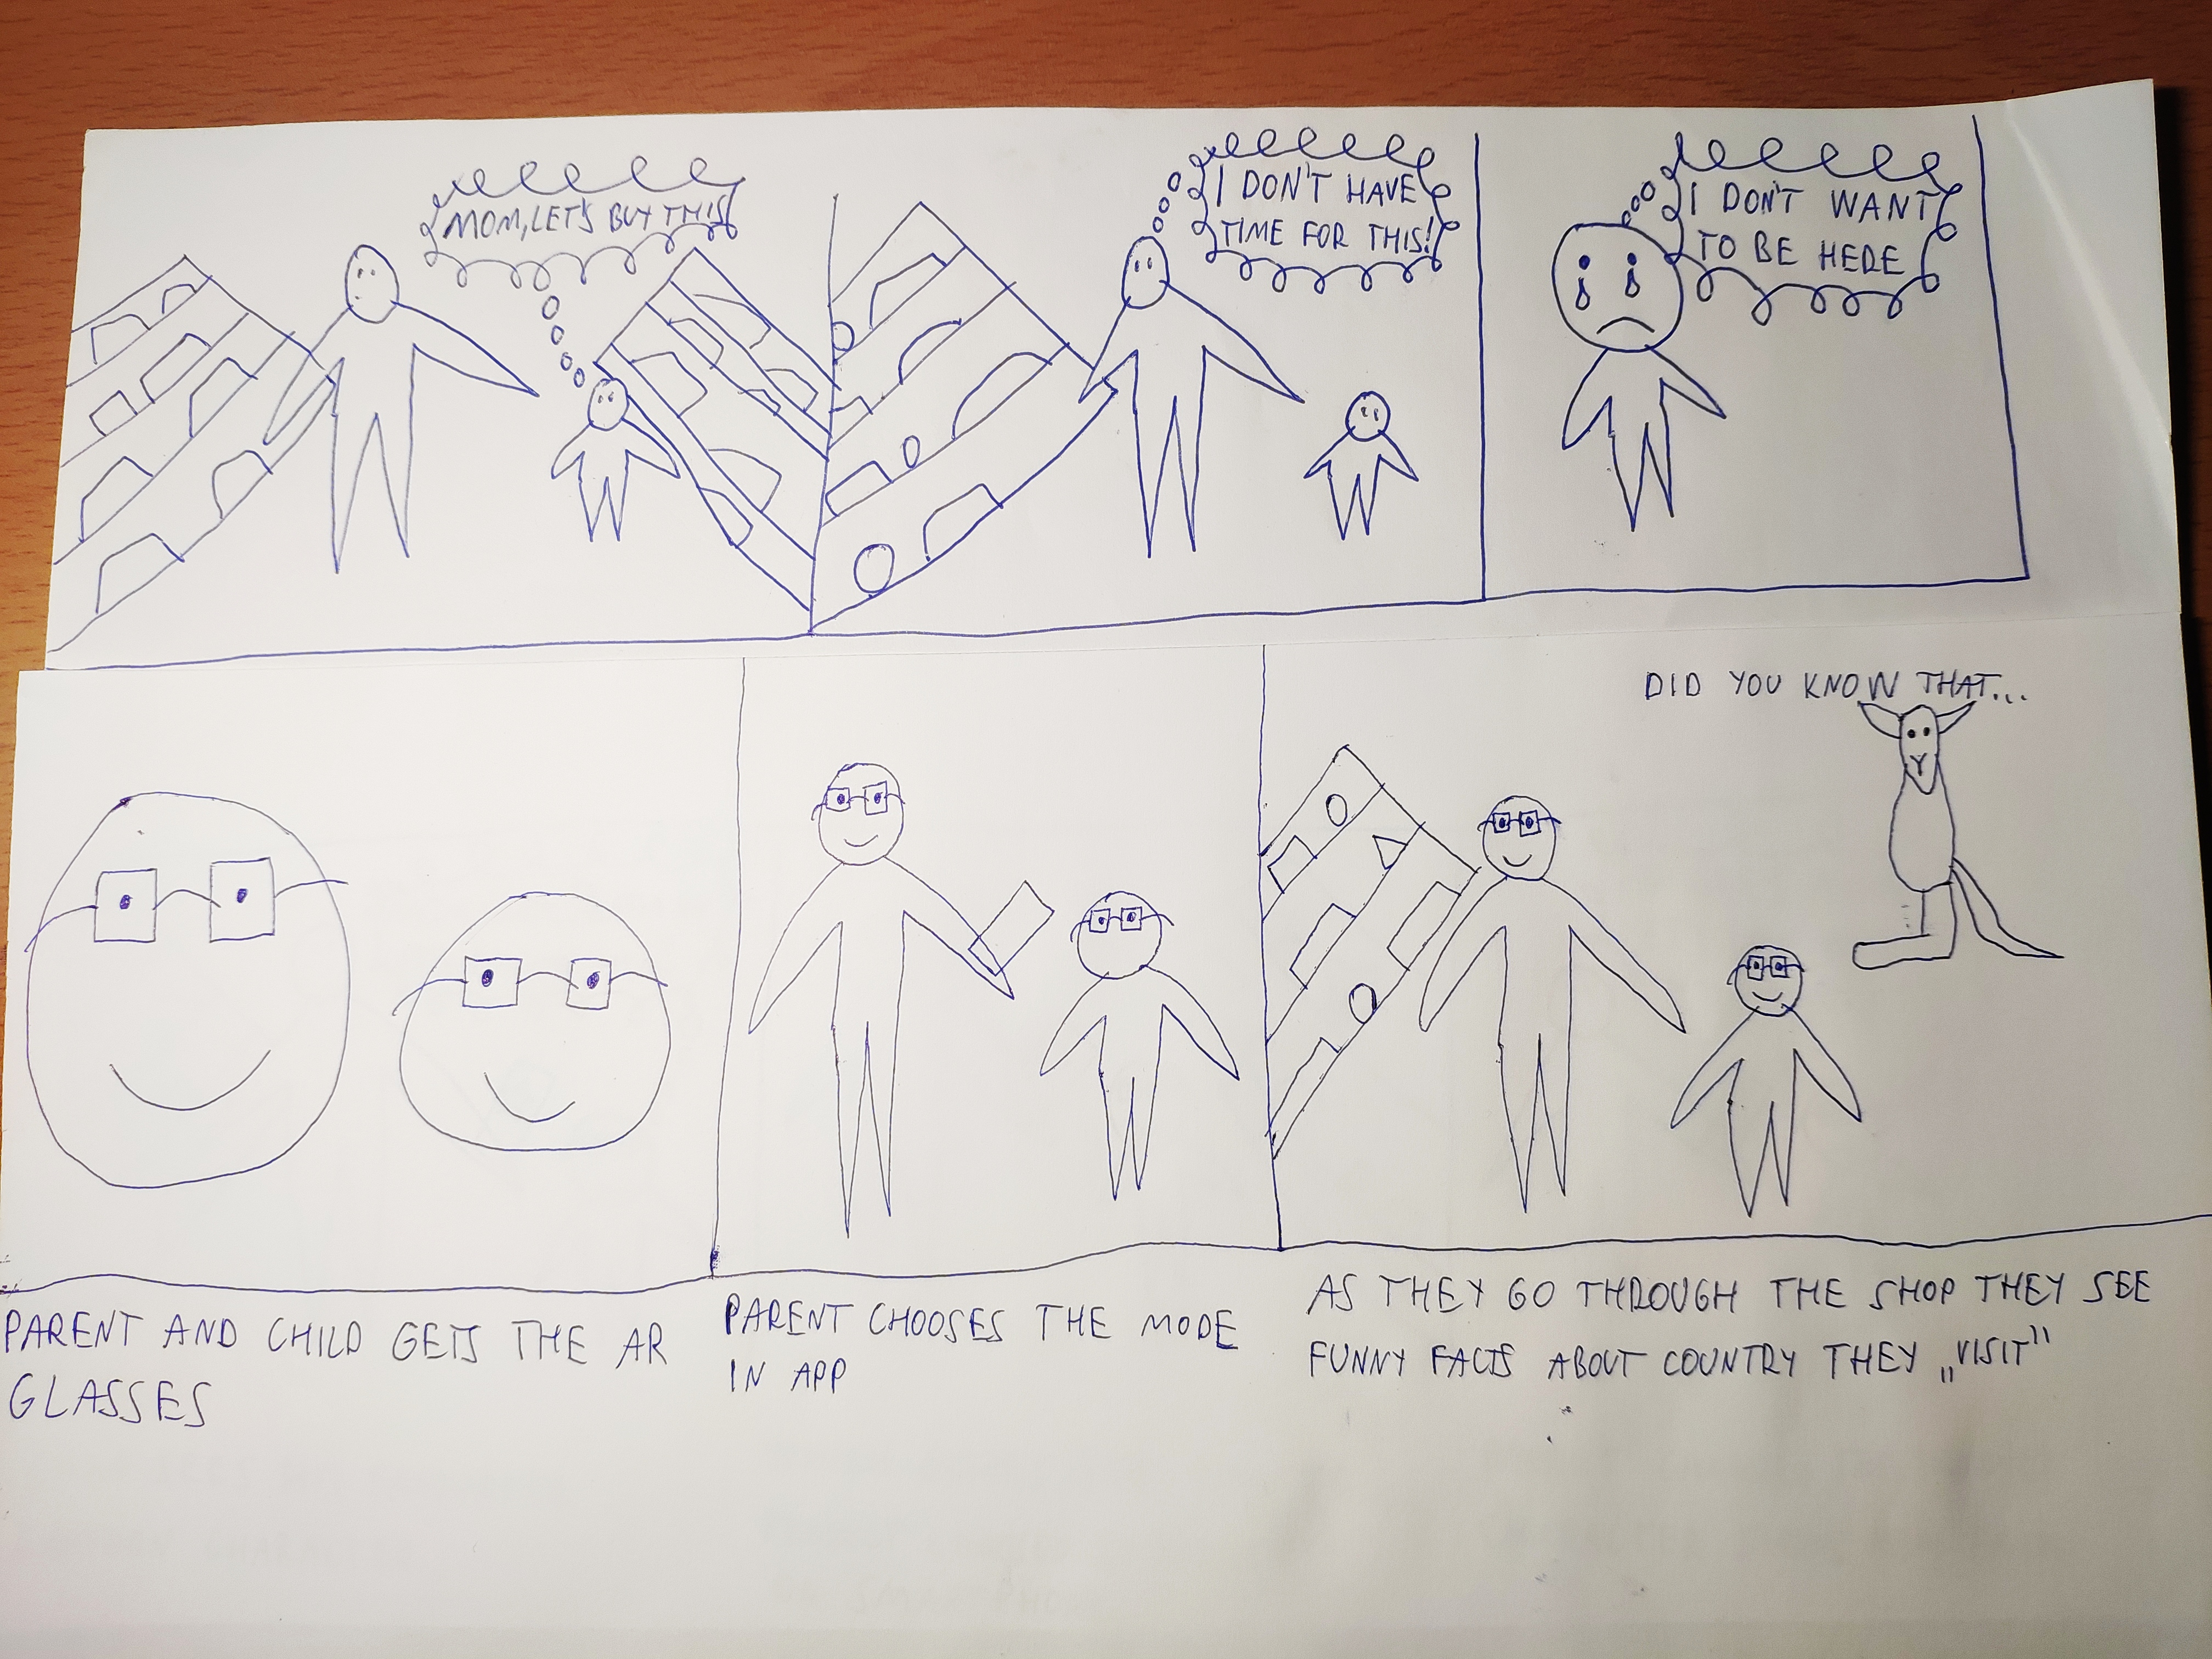
\includegraphics[scale=0.16, clip, trim={40em 28em 40em 33em}]{images/s1.jpg}
\end{figure}

User \#1:
\begin{compactitem}
	\item Name: Hakan
	\item Information: age of 23, Turkish
	\item Profession: M.Sc. student
	\item likes to  play games and hang out with friends
	\item representative of our third persona (David)
\end{compactitem}
\bigskip

Answers:
\begin{compactitem}
	\item Do the users understand the solution?\\
		Yes, it was clear for the user. The user also really likes the solution.\\
	
	\item Do the users find the solution realistic?\\
		Not so much. The other parts are really possible, while VR goggles part was not realistic at all: the fighting with the other mascots is silly, not everyone wants that (might be hard for elderly). But fighting for right-earned food might also be fun for some.\\
		
	\item Do the users feel that this solution can solve his/her problem(s)? If not, what is still
	a problem? Is there a solution that could solve this?\\
		Yes, especially when he wants to find some obscure ingredient that he needs to complete a recipe. It is also better than asking some retail worker. He agreed that it might solve his problem.
\end{compactitem}

\bigskip
\bigskip

User \#2:
\begin{compactitem}
	\item Name: Furkan
	\item Information: age of 26, Turkish
	\item Profession: M.Sc. student
	\item interested in fitness, likes to learn about anything, joining online courses, gym-going, reading a lot
	\item representative of our first persona (Picky Eater Helga Ratt)
\end{compactitem}
\bigskip

Answers:
\begin{compactitem}
	\item Do the users understand the solution?\\
		Yes, only the game part is not very clear. How is he going to kill the other mascots was not clear. One other question was whether VR goggles are going to provided by the market.\\
	
	\item Do the users find the solution realistic?\\
	He is both concerned about the number of available screens in the market and who would provide the VR goggles. In short, he does not find it that much realistic.\\
	
	\item Do the users feel that this solution can solve his/her problem(s)? If not, what is still
	a problem? Is there a solution that could solve this?\\
		He thinks this would not solve his problems in its current form. He would like to have it in a way that more than one item is searchable via the application, so we would not spend so much time in front of the screen. However, he finds this promising.\\
		(he is also curious whether people would be concerned about gazes of others, as this application would be out in the open and everyone would see what he searched for)\\
		He said playing games in home and coming to fetch the coupons would be more fun!
\end{compactitem}

\clearpage

\section{Solution \#2:}
\begin{figure}[h]
	\centering
	\includegraphics[scale=0.16, clip, trim={71em 35em 33em 43em}]{images/s2.jpg}
\end{figure}

User \#1:
\begin{compactitem}
	\item Name: Hakan
	\item Information: age of 23, Turkish
	\item Profession: M.Sc. student
	\item likes to  play games and hang out with friends
	\item representative of our third persona (David)
\end{compactitem}
\bigskip

Answers:
\begin{compactitem}
	\item Do the users understand the solution?\\
	Yes, it is quite clear. The user were able to explain the solution completely by putting himself in the shoes of the example in the storyboard.\\
	
	\item Do the users find the solution realistic?\\
	Much more realistic than the Solution \#1. Also, he finds this solution innovative to come up with.\\
	
	\item Do the users feel that this solution can solve his/her problem(s)? If not, what is still
	a problem? Is there a solution that could solve this?\\
	Yes, definitely. He also goes around the shop and got bored afterwards seeing all the same places, and this would really improve his experience.\\
\end{compactitem}

\bigskip
\bigskip

User \#2:
\begin{compactitem}
	\item Name: Furkan
	\item Information: age of 26, Turkish
	\item Profession: M.Sc. student
	\item interested in fitness, likes to learn about anything, joining online courses, gym-going, reading a lot
	\item representative of our first persona (Picky Eater Helga Ratt)
\end{compactitem}
\bigskip

Answers:
\begin{compactitem}
	\item Do the users understand the solution?\\

	
	\item Do the users find the solution realistic?\\
	
	
	\item Do the users feel that this solution can solve his/her problem(s)? If not, what is still
	a problem? Is there a solution that could solve this?\\
\end{compactitem}

\clearpage
\section{Solution \#3:}

\clearpage
\section{Solution \#4:}

\clearpage
\section{Solution \#5:}

\clearpage
\section{Solution \#6:}

\chapter{Our Evaluation}

Selected Solutions:\\

\section{Solution \#x:}

\section{Solution \#y:}

\section{Solution \#z:}

\chapter{Final Storyboards}
				
\end{document}}
